% Options for packages loaded elsewhere
\PassOptionsToPackage{unicode}{hyperref}
\PassOptionsToPackage{hyphens}{url}
\PassOptionsToPackage{dvipsnames,svgnames,x11names}{xcolor}
%
\documentclass[
  letterpaper,
  DIV=11,
  numbers=noendperiod]{scrreprt}

\usepackage{amsmath,amssymb}
\usepackage{lmodern}
\usepackage{iftex}
\ifPDFTeX
  \usepackage[T1]{fontenc}
  \usepackage[utf8]{inputenc}
  \usepackage{textcomp} % provide euro and other symbols
\else % if luatex or xetex
  \usepackage{unicode-math}
  \defaultfontfeatures{Scale=MatchLowercase}
  \defaultfontfeatures[\rmfamily]{Ligatures=TeX,Scale=1}
\fi
% Use upquote if available, for straight quotes in verbatim environments
\IfFileExists{upquote.sty}{\usepackage{upquote}}{}
\IfFileExists{microtype.sty}{% use microtype if available
  \usepackage[]{microtype}
  \UseMicrotypeSet[protrusion]{basicmath} % disable protrusion for tt fonts
}{}
\makeatletter
\@ifundefined{KOMAClassName}{% if non-KOMA class
  \IfFileExists{parskip.sty}{%
    \usepackage{parskip}
  }{% else
    \setlength{\parindent}{0pt}
    \setlength{\parskip}{6pt plus 2pt minus 1pt}}
}{% if KOMA class
  \KOMAoptions{parskip=half}}
\makeatother
\usepackage{xcolor}
\setlength{\emergencystretch}{3em} % prevent overfull lines
\setcounter{secnumdepth}{-\maxdimen} % remove section numbering
% Make \paragraph and \subparagraph free-standing
\ifx\paragraph\undefined\else
  \let\oldparagraph\paragraph
  \renewcommand{\paragraph}[1]{\oldparagraph{#1}\mbox{}}
\fi
\ifx\subparagraph\undefined\else
  \let\oldsubparagraph\subparagraph
  \renewcommand{\subparagraph}[1]{\oldsubparagraph{#1}\mbox{}}
\fi

\usepackage{color}
\usepackage{fancyvrb}
\newcommand{\VerbBar}{|}
\newcommand{\VERB}{\Verb[commandchars=\\\{\}]}
\DefineVerbatimEnvironment{Highlighting}{Verbatim}{commandchars=\\\{\}}
% Add ',fontsize=\small' for more characters per line
\usepackage{framed}
\definecolor{shadecolor}{RGB}{241,243,245}
\newenvironment{Shaded}{\begin{snugshade}}{\end{snugshade}}
\newcommand{\AlertTok}[1]{\textcolor[rgb]{0.68,0.00,0.00}{#1}}
\newcommand{\AnnotationTok}[1]{\textcolor[rgb]{0.37,0.37,0.37}{#1}}
\newcommand{\AttributeTok}[1]{\textcolor[rgb]{0.40,0.45,0.13}{#1}}
\newcommand{\BaseNTok}[1]{\textcolor[rgb]{0.68,0.00,0.00}{#1}}
\newcommand{\BuiltInTok}[1]{\textcolor[rgb]{0.00,0.23,0.31}{#1}}
\newcommand{\CharTok}[1]{\textcolor[rgb]{0.13,0.47,0.30}{#1}}
\newcommand{\CommentTok}[1]{\textcolor[rgb]{0.37,0.37,0.37}{#1}}
\newcommand{\CommentVarTok}[1]{\textcolor[rgb]{0.37,0.37,0.37}{\textit{#1}}}
\newcommand{\ConstantTok}[1]{\textcolor[rgb]{0.56,0.35,0.01}{#1}}
\newcommand{\ControlFlowTok}[1]{\textcolor[rgb]{0.00,0.23,0.31}{#1}}
\newcommand{\DataTypeTok}[1]{\textcolor[rgb]{0.68,0.00,0.00}{#1}}
\newcommand{\DecValTok}[1]{\textcolor[rgb]{0.68,0.00,0.00}{#1}}
\newcommand{\DocumentationTok}[1]{\textcolor[rgb]{0.37,0.37,0.37}{\textit{#1}}}
\newcommand{\ErrorTok}[1]{\textcolor[rgb]{0.68,0.00,0.00}{#1}}
\newcommand{\ExtensionTok}[1]{\textcolor[rgb]{0.00,0.23,0.31}{#1}}
\newcommand{\FloatTok}[1]{\textcolor[rgb]{0.68,0.00,0.00}{#1}}
\newcommand{\FunctionTok}[1]{\textcolor[rgb]{0.28,0.35,0.67}{#1}}
\newcommand{\ImportTok}[1]{\textcolor[rgb]{0.00,0.46,0.62}{#1}}
\newcommand{\InformationTok}[1]{\textcolor[rgb]{0.37,0.37,0.37}{#1}}
\newcommand{\KeywordTok}[1]{\textcolor[rgb]{0.00,0.23,0.31}{#1}}
\newcommand{\NormalTok}[1]{\textcolor[rgb]{0.00,0.23,0.31}{#1}}
\newcommand{\OperatorTok}[1]{\textcolor[rgb]{0.37,0.37,0.37}{#1}}
\newcommand{\OtherTok}[1]{\textcolor[rgb]{0.00,0.23,0.31}{#1}}
\newcommand{\PreprocessorTok}[1]{\textcolor[rgb]{0.68,0.00,0.00}{#1}}
\newcommand{\RegionMarkerTok}[1]{\textcolor[rgb]{0.00,0.23,0.31}{#1}}
\newcommand{\SpecialCharTok}[1]{\textcolor[rgb]{0.37,0.37,0.37}{#1}}
\newcommand{\SpecialStringTok}[1]{\textcolor[rgb]{0.13,0.47,0.30}{#1}}
\newcommand{\StringTok}[1]{\textcolor[rgb]{0.13,0.47,0.30}{#1}}
\newcommand{\VariableTok}[1]{\textcolor[rgb]{0.07,0.07,0.07}{#1}}
\newcommand{\VerbatimStringTok}[1]{\textcolor[rgb]{0.13,0.47,0.30}{#1}}
\newcommand{\WarningTok}[1]{\textcolor[rgb]{0.37,0.37,0.37}{\textit{#1}}}

\providecommand{\tightlist}{%
  \setlength{\itemsep}{0pt}\setlength{\parskip}{0pt}}\usepackage{longtable,booktabs,array}
\usepackage{calc} % for calculating minipage widths
% Correct order of tables after \paragraph or \subparagraph
\usepackage{etoolbox}
\makeatletter
\patchcmd\longtable{\par}{\if@noskipsec\mbox{}\fi\par}{}{}
\makeatother
% Allow footnotes in longtable head/foot
\IfFileExists{footnotehyper.sty}{\usepackage{footnotehyper}}{\usepackage{footnote}}
\makesavenoteenv{longtable}
\usepackage{graphicx}
\makeatletter
\def\maxwidth{\ifdim\Gin@nat@width>\linewidth\linewidth\else\Gin@nat@width\fi}
\def\maxheight{\ifdim\Gin@nat@height>\textheight\textheight\else\Gin@nat@height\fi}
\makeatother
% Scale images if necessary, so that they will not overflow the page
% margins by default, and it is still possible to overwrite the defaults
% using explicit options in \includegraphics[width, height, ...]{}
\setkeys{Gin}{width=\maxwidth,height=\maxheight,keepaspectratio}
% Set default figure placement to htbp
\makeatletter
\def\fps@figure{htbp}
\makeatother

\KOMAoption{captions}{tableheading,figureheading}
\makeatletter
\makeatother
\makeatletter
\makeatother
\makeatletter
\@ifpackageloaded{caption}{}{\usepackage{caption}}
\AtBeginDocument{%
\ifdefined\contentsname
  \renewcommand*\contentsname{Table of contents}
\else
  \newcommand\contentsname{Table of contents}
\fi
\ifdefined\listfigurename
  \renewcommand*\listfigurename{List of Figures}
\else
  \newcommand\listfigurename{List of Figures}
\fi
\ifdefined\listtablename
  \renewcommand*\listtablename{List of Tables}
\else
  \newcommand\listtablename{List of Tables}
\fi
\ifdefined\figurename
  \renewcommand*\figurename{Figure}
\else
  \newcommand\figurename{Figure}
\fi
\ifdefined\tablename
  \renewcommand*\tablename{Table}
\else
  \newcommand\tablename{Table}
\fi
}
\@ifpackageloaded{float}{}{\usepackage{float}}
\floatstyle{ruled}
\@ifundefined{c@chapter}{\newfloat{codelisting}{h}{lop}}{\newfloat{codelisting}{h}{lop}[chapter]}
\floatname{codelisting}{Listing}
\newcommand*\listoflistings{\listof{codelisting}{List of Listings}}
\makeatother
\makeatletter
\@ifpackageloaded{caption}{}{\usepackage{caption}}
\@ifpackageloaded{subcaption}{}{\usepackage{subcaption}}
\makeatother
\makeatletter
\@ifpackageloaded{tcolorbox}{}{\usepackage[many]{tcolorbox}}
\makeatother
\makeatletter
\@ifundefined{shadecolor}{\definecolor{shadecolor}{rgb}{.97, .97, .97}}
\makeatother
\makeatletter
\makeatother
\ifLuaTeX
  \usepackage{selnolig}  % disable illegal ligatures
\fi
\IfFileExists{bookmark.sty}{\usepackage{bookmark}}{\usepackage{hyperref}}
\IfFileExists{xurl.sty}{\usepackage{xurl}}{} % add URL line breaks if available
\urlstyle{same} % disable monospaced font for URLs
\hypersetup{
  colorlinks=true,
  linkcolor={blue},
  filecolor={Maroon},
  citecolor={Blue},
  urlcolor={Blue},
  pdfcreator={LaTeX via pandoc}}

\author{}
\date{}

\begin{document}
\ifdefined\Shaded\renewenvironment{Shaded}{\begin{tcolorbox}[enhanced, sharp corners, breakable, boxrule=0pt, interior hidden, borderline west={3pt}{0pt}{shadecolor}, frame hidden]}{\end{tcolorbox}}\fi

\hypertarget{introduction-to-using-r}{%
\chapter*{Introduction to Using R}\label{introduction-to-using-r}}
\addcontentsline{toc}{chapter}{Introduction to Using R}

\hypertarget{introduction}{%
\section{Introduction}\label{introduction}}

R is an object-oriented programming language like
\href{https://www.python.org/}{Python},
\href{https://julialang.org/}{Julia}, and
\href{https://www.javascript.com/}{JavaScript}. Like these programming
languages, R has a specific syntax or function, which is essential to
understand if you want to use its features to accomplish thousands of
things with R. However, one of the most challenging parts of learning R
is finding your way around. In section of tutorial you will learn some
basic of R such as syntax of R programming, assignment statements,
r-data types, control statements and simple r-function.

\hypertarget{screen-prompt}{%
\section{Screen Prompt}\label{screen-prompt}}

The \textbf{screen prompt \textgreater{}} in R-console is an place to
put command or instruction for R to work. Press the ``Ctrl'' + ``L''
keys simultaneously. The screen will now be refreshed and the console
should be cleared.

\begin{figure}

\caption{\label{fig-screen_prompt}R Screen Prompt}

{\centering 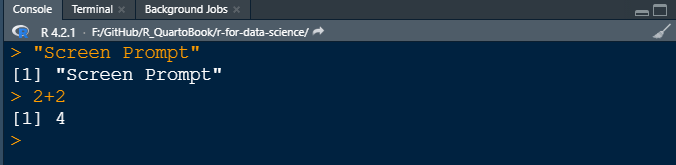
\includegraphics{Image/sreen_prompt.png}

}

\end{figure}

\hypertarget{r-as-a-calculator}{%
\section{R as a Calculator}\label{r-as-a-calculator}}

We can use R as a calculators, at the prompt, we enter the expression
that we want evaluated and when we hit enter, it will compute the result
for us . For Example:

For addition:

\begin{Shaded}
\begin{Highlighting}[]
\DecValTok{2}\SpecialCharTok{+}\DecValTok{2}
\end{Highlighting}
\end{Shaded}

\begin{verbatim}
[1] 4
\end{verbatim}

And for subtraction:

\begin{Shaded}
\begin{Highlighting}[]
\DecValTok{4{-}2}
\end{Highlighting}
\end{Shaded}

\begin{verbatim}
[1] 2
\end{verbatim}

For multiplication:

\begin{Shaded}
\begin{Highlighting}[]
\DecValTok{4}\SpecialCharTok{*}\DecValTok{2}
\end{Highlighting}
\end{Shaded}

\begin{verbatim}
[1] 8
\end{verbatim}

For raised to the power:

\begin{Shaded}
\begin{Highlighting}[]
\DecValTok{2}\SpecialCharTok{\^{}}\DecValTok{2}
\end{Highlighting}
\end{Shaded}

\begin{verbatim}
[1] 4
\end{verbatim}

Use parentheses to ensure that it understands what you are trying to
compute.

https://www.geeksforgeeks.org/control-statements-in-r-programming/?ref=lbp

\hypertarget{syntax-of-r-program}{%
\section{Syntax of R program}\label{syntax-of-r-program}}

\textbf{Variables}, \textbf{Comments}, and \textbf{Keywords} are the
three main components in R- programming. Variables are used to store the
data, Comments are used to improve code readability, and Keywords are
reserved words that hold a specific meaning to the compiler.

\hypertarget{built-in-function}{%
\section{Built in Function}\label{built-in-function}}

There are so many built-in mathematical functions are available in
base-R. Some are shown in below table:

\begin{figure}

\caption{Built-in Math Functions}

{\centering 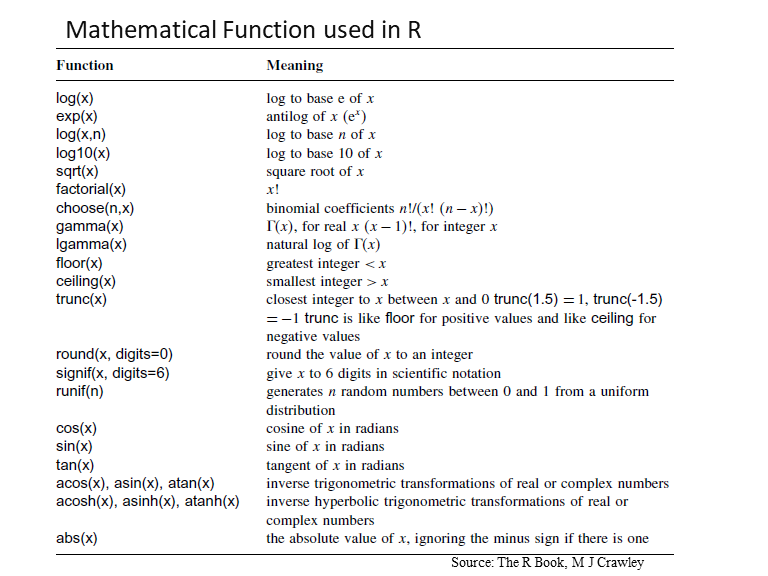
\includegraphics{Image/Table_math_function.png}

}

\end{figure}

Here below some examples of R built-in R-functions

\begin{Shaded}
\begin{Highlighting}[]
\FunctionTok{log10}\NormalTok{(}\DecValTok{2}\NormalTok{)}
\end{Highlighting}
\end{Shaded}

\begin{verbatim}
[1] 0.30103
\end{verbatim}

\begin{Shaded}
\begin{Highlighting}[]
\FunctionTok{exp}\NormalTok{(}\DecValTok{1}\NormalTok{)}
\end{Highlighting}
\end{Shaded}

\begin{verbatim}
[1] 2.718282
\end{verbatim}

\begin{Shaded}
\begin{Highlighting}[]
\NormalTok{pi}
\end{Highlighting}
\end{Shaded}

\begin{verbatim}
[1] 3.141593
\end{verbatim}

\begin{Shaded}
\begin{Highlighting}[]
\FunctionTok{sin}\NormalTok{(pi}\SpecialCharTok{/}\DecValTok{2}\NormalTok{)}
\end{Highlighting}
\end{Shaded}

\begin{verbatim}
[1] 1
\end{verbatim}

\hypertarget{number-with-exponents}{%
\section{Number with Exponents}\label{number-with-exponents}}

We can use very big numbers or very small numbers in R using the
following scheme:

\begin{Shaded}
\begin{Highlighting}[]
\FloatTok{1.2e3} \CommentTok{\# means 1200 because the e3 means ‘move the decimal point 3 places to the right }
\end{Highlighting}
\end{Shaded}

\begin{verbatim}
[1] 1200
\end{verbatim}

\begin{Shaded}
\begin{Highlighting}[]
\FloatTok{1.2e{-}2} \CommentTok{\# means 0.012 because the e{-}2 means ‘move the decimal point 2 places to the left’}
\end{Highlighting}
\end{Shaded}

\begin{verbatim}
[1] 0.012
\end{verbatim}

\hypertarget{modulo-and-integer-quotients}{%
\section{Modulo and Integer
Quotients}\label{modulo-and-integer-quotients}}

Suppose we want to know the integer part of a division: say, how many
13s are there in 119:

\begin{Shaded}
\begin{Highlighting}[]
\DecValTok{119} \SpecialCharTok{\%/\%} \DecValTok{13}
\end{Highlighting}
\end{Shaded}

\begin{verbatim}
[1] 9
\end{verbatim}

Suppose we wanted to know the remainder (what is left over when 119 is
divided by 13: in maths this is known as modulo

\begin{Shaded}
\begin{Highlighting}[]
\DecValTok{119} \SpecialCharTok{\%\%} \DecValTok{13}
\end{Highlighting}
\end{Shaded}

\begin{verbatim}
[1] 2
\end{verbatim}

\hypertarget{rounding}{%
\section{Rounding}\label{rounding}}

Several types of rounding (rounding up, rounding down, rounding to the
nearest integer) can be done easily with R.

The `greatest integer less than' function is \textbf{floor()}

\begin{Shaded}
\begin{Highlighting}[]
\FunctionTok{floor}\NormalTok{(}\FloatTok{5.7}\NormalTok{)}
\end{Highlighting}
\end{Shaded}

\begin{verbatim}
[1] 5
\end{verbatim}

The `next integer' function is \textbf{ceiling}()

\begin{Shaded}
\begin{Highlighting}[]
\FunctionTok{ceiling}\NormalTok{(}\FloatTok{5.7}\NormalTok{)}
\end{Highlighting}
\end{Shaded}

\begin{verbatim}
[1] 6
\end{verbatim}

\hypertarget{assignment-statements}{%
\section{Assignment Statements}\label{assignment-statements}}

Just like in algebra, we often want to store a computation under some
variable name. The result is assigned to a variable with the symbols =
or \textless- which is formed by the ``less than'' symbol followed
immediately by a hyphen.

\begin{Shaded}
\begin{Highlighting}[]
\NormalTok{x}\OtherTok{\textless{}{-}}\DecValTok{10}\NormalTok{; }\CommentTok{\# or}
\NormalTok{y }\OtherTok{=} \DecValTok{12}
\end{Highlighting}
\end{Shaded}

When you want to know what is in a variable simply ask by typing the
variable name.

\begin{Shaded}
\begin{Highlighting}[]
\NormalTok{x; }\CommentTok{\# or}
\end{Highlighting}
\end{Shaded}

\begin{verbatim}
[1] 10
\end{verbatim}

\begin{Shaded}
\begin{Highlighting}[]
\NormalTok{y}
\end{Highlighting}
\end{Shaded}

\begin{verbatim}
[1] 12
\end{verbatim}

We can store a computation of two variable names and do some calculation
and the result is assigned to a new variable

\begin{Shaded}
\begin{Highlighting}[]
\NormalTok{a}\OtherTok{=}\DecValTok{2}\NormalTok{;}
\NormalTok{b}\OtherTok{=}\DecValTok{3}\NormalTok{;}
\NormalTok{c}\OtherTok{=}\NormalTok{a}\SpecialCharTok{+}\NormalTok{b;}
\NormalTok{c}
\end{Highlighting}
\end{Shaded}

\begin{verbatim}
[1] 5
\end{verbatim}

\hypertarget{variable-names}{%
\section{Variable Names}\label{variable-names}}

\begin{itemize}
\item
  Do not begin a variable name with a period or a number. Variable names
  are case (upper/lower) sensitive.
\item
  Variable names in R are case-sensitive so x is not the same as X.
\item
  Variable names should not begin with numbers (e.g.~1x) or symbols
  (e.g.~\%x).
\item
  Variable names should not contain blank spaces: use grain.yield
\end{itemize}

\hypertarget{operators}{%
\section{Operators}\label{operators}}

\begin{Shaded}
\begin{Highlighting}[]
\CommentTok{\# + {-} */\%\% \^{} arithmetic}
\CommentTok{\# \textgreater{} \textgreater{}= \textless{} \textless{}= == != relational}
\CommentTok{\# ! \&  logical}
\CommentTok{\# \textasciitilde{} model formulae}
\CommentTok{\# \textless{}{-} {-}\textgreater{} assignment}
\CommentTok{\# $ list indexing (the ‘element name’ operator)}
\CommentTok{\# : create a sequence}
\end{Highlighting}
\end{Shaded}

\hypertarget{r-data-types}{%
\section{R Data Types}\label{r-data-types}}

R has a wide variety of data types including scalars, vectors
(numerical, character, logical), matrices, data frames, and lists.

\hypertarget{vectors}{%
\subsection{Vectors}\label{vectors}}

Vectors is data-type with one or more values of the same type such as
logical, integer, real, complex, string (or character) or raw vectors.
Unlike Python, the indexing of the vector in R will start from `1' and
not from `0'.

A scalar data structure is the most basic data type that holds only a
\textbf{single atomic value} at a time. Using scalars, more complex data
types can be constructed. The most commonly used scalar types in R:

\begin{itemize}
\item
  Numeric
\item
  Character or strings
\item
  Integer
\item
  Logical
\item
  Complex
\end{itemize}

\textbf{Numeric} is the default type used in R for mathematical
computations. Examples of numeric are decimal numbers and whole numbers.

\begin{Shaded}
\begin{Highlighting}[]
\NormalTok{x}\OtherTok{=}\FloatTok{1.2}
\NormalTok{x}
\end{Highlighting}
\end{Shaded}

\begin{verbatim}
[1] 1.2
\end{verbatim}

\begin{Shaded}
\begin{Highlighting}[]
\FunctionTok{class}\NormalTok{(x)}
\end{Highlighting}
\end{Shaded}

\begin{verbatim}
[1] "numeric"
\end{verbatim}

\textbf{Character} objects are \textbf{strings}. They could be any
sequence of characters including alphabets, numbers, punctuation marks,
etc. enclosed in quotes.

\begin{Shaded}
\begin{Highlighting}[]
\NormalTok{Department }\OtherTok{=} \StringTok{\textquotesingle{}Chemistry\textquotesingle{}}
\NormalTok{School}\OtherTok{=} \StringTok{"University at Buffalo"}
\FunctionTok{class}\NormalTok{(School)}
\end{Highlighting}
\end{Shaded}

\begin{verbatim}
[1] "character"
\end{verbatim}

\begin{Shaded}
\begin{Highlighting}[]
\FunctionTok{paste}\NormalTok{(Department,}\StringTok{","}\NormalTok{, School)}
\end{Highlighting}
\end{Shaded}

\begin{verbatim}
[1] "Chemistry , University at Buffalo"
\end{verbatim}

\textbf{Logical} values are \textbf{boolean} values of \textbf{TRUE} or
\textbf{FALSE}. Note that R needs logical values of TRUE or FALSE to be
in upper case. If you use mixed case or lowercase, you'll get an error
or unpredictable results.

\begin{Shaded}
\begin{Highlighting}[]
\NormalTok{u }\OtherTok{=} \ConstantTok{TRUE}\NormalTok{; }
\NormalTok{v }\OtherTok{=} \ConstantTok{FALSE}
\FunctionTok{class}\NormalTok{(u)}
\end{Highlighting}
\end{Shaded}

\begin{verbatim}
[1] "logical"
\end{verbatim}

\begin{Shaded}
\begin{Highlighting}[]
\FunctionTok{class}\NormalTok{(v)}
\end{Highlighting}
\end{Shaded}

\begin{verbatim}
[1] "logical"
\end{verbatim}

A list of numbers or charterers together to form a \textbf{Multiple
Elements Vector}. Values can be assigned to vectors in many different
ways. We can create a vector of number from 1 to 10, using the
concatenation function \textbf{c}

\begin{Shaded}
\begin{Highlighting}[]
\NormalTok{a }\OtherTok{\textless{}{-}} \FunctionTok{c}\NormalTok{(}\DecValTok{1}\NormalTok{,}\DecValTok{2}\NormalTok{,}\FloatTok{5.3}\NormalTok{,}\DecValTok{6}\NormalTok{,}\DecValTok{7}\NormalTok{,}\DecValTok{8}\NormalTok{,}\DecValTok{9}\NormalTok{,}\DecValTok{10}\NormalTok{)}
\NormalTok{a}
\end{Highlighting}
\end{Shaded}

\begin{verbatim}
[1]  1.0  2.0  5.3  6.0  7.0  8.0  9.0 10.0
\end{verbatim}

\begin{Shaded}
\begin{Highlighting}[]
\NormalTok{s }\OtherTok{\textless{}{-}} \FunctionTok{c}\NormalTok{(}\StringTok{\textquotesingle{}apple\textquotesingle{}}\NormalTok{,}\StringTok{\textquotesingle{}red\textquotesingle{}}\NormalTok{,}\DecValTok{5}\NormalTok{,}\ConstantTok{TRUE}\NormalTok{)}
\FunctionTok{print}\NormalTok{(s)}
\end{Highlighting}
\end{Shaded}

\begin{verbatim}
[1] "apple" "red"   "5"     "TRUE" 
\end{verbatim}

It can be generated by the sequence of integer values 1 to 10 using :
(colon), the sequence-generating operator,

\begin{Shaded}
\begin{Highlighting}[]
\NormalTok{a}\OtherTok{\textless{}{-}}\DecValTok{1}\SpecialCharTok{:}\DecValTok{10}
\NormalTok{a}
\end{Highlighting}
\end{Shaded}

\begin{verbatim}
 [1]  1  2  3  4  5  6  7  8  9 10
\end{verbatim}

We can also create a vector using Using sequence (Seq.) operator.

\begin{Shaded}
\begin{Highlighting}[]
\CommentTok{\# Create vector with elements from 5 to 9 incrementing by 0.4.}
\NormalTok{b }\OtherTok{=} \FunctionTok{seq}\NormalTok{(}\DecValTok{5}\NormalTok{, }\DecValTok{9}\NormalTok{, }\AttributeTok{by =} \FloatTok{0.4}\NormalTok{)}
\NormalTok{b}
\end{Highlighting}
\end{Shaded}

\begin{verbatim}
 [1] 5.0 5.4 5.8 6.2 6.6 7.0 7.4 7.8 8.2 8.6 9.0
\end{verbatim}

R has ability to evaluate functions over entire vectors, so no need to
write , for loops and subscripts. Important vector functions are listed
in below Table:

\begin{figure}

\caption{Vector Functions}

{\centering 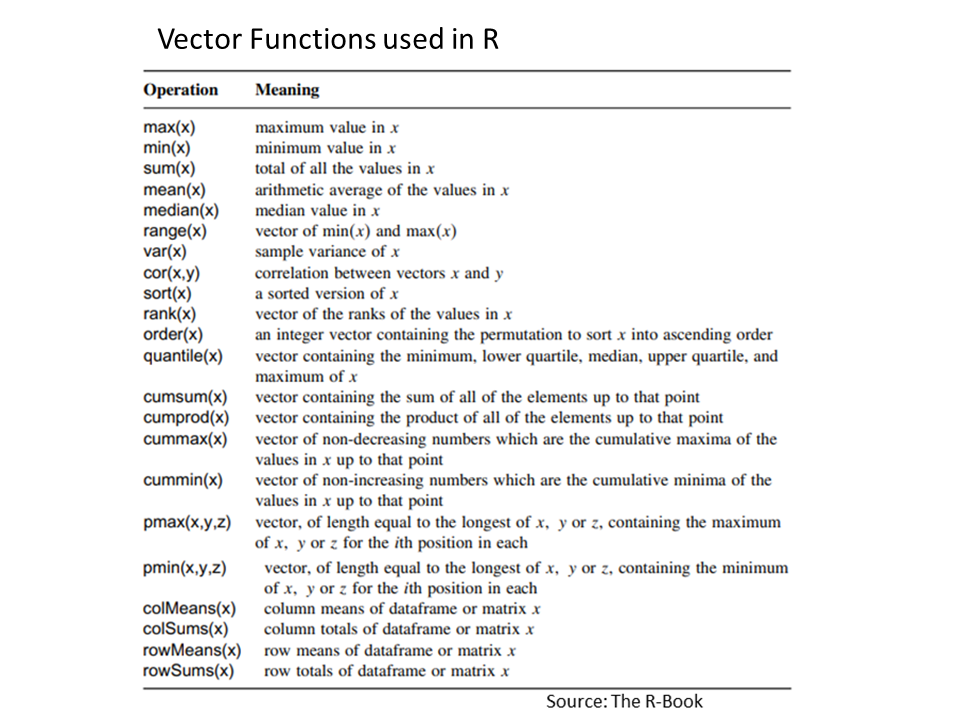
\includegraphics{Image/vector_functions.png}

}

\end{figure}

Once we have a vector of numbers we can apply certain built-in functions
to them to get useful summaries. For example:

\begin{Shaded}
\begin{Highlighting}[]
\FunctionTok{sum}\NormalTok{(a)        }\CommentTok{\# sums the values in the vector }
\end{Highlighting}
\end{Shaded}

\begin{verbatim}
[1] 55
\end{verbatim}

\begin{Shaded}
\begin{Highlighting}[]
\FunctionTok{length}\NormalTok{(a)     }\CommentTok{\# number of the values in the vector }
\end{Highlighting}
\end{Shaded}

\begin{verbatim}
[1] 10
\end{verbatim}

\begin{Shaded}
\begin{Highlighting}[]
\FunctionTok{mean}\NormalTok{ (a)      }\CommentTok{\# the average of the values in the vector }
\end{Highlighting}
\end{Shaded}

\begin{verbatim}
[1] 5.5
\end{verbatim}

\begin{Shaded}
\begin{Highlighting}[]
\FunctionTok{var}\NormalTok{ (a)        }\CommentTok{\# the sample variance of the values }
\end{Highlighting}
\end{Shaded}

\begin{verbatim}
[1] 9.166667
\end{verbatim}

\begin{Shaded}
\begin{Highlighting}[]
\FunctionTok{sd}\NormalTok{(a)         }\CommentTok{\# the standard of deviations of the values  }
\end{Highlighting}
\end{Shaded}

\begin{verbatim}
[1] 3.02765
\end{verbatim}

\begin{Shaded}
\begin{Highlighting}[]
\FunctionTok{max}\NormalTok{(a)        }\CommentTok{\# the largest value in the vector  }
\end{Highlighting}
\end{Shaded}

\begin{verbatim}
[1] 10
\end{verbatim}

\begin{Shaded}
\begin{Highlighting}[]
\FunctionTok{min}\NormalTok{(a)        }\CommentTok{\# the smallest number in the vector }
\end{Highlighting}
\end{Shaded}

\begin{verbatim}
[1] 1
\end{verbatim}

\begin{Shaded}
\begin{Highlighting}[]
\FunctionTok{median}\NormalTok{(a)     }\CommentTok{\# the sample median }
\end{Highlighting}
\end{Shaded}

\begin{verbatim}
[1] 5.5
\end{verbatim}

\textbf{Summary()} function will calculate summary statistics of a
vector

\begin{Shaded}
\begin{Highlighting}[]
\FunctionTok{summary}\NormalTok{(a)}
\end{Highlighting}
\end{Shaded}

\begin{verbatim}
   Min. 1st Qu.  Median    Mean 3rd Qu.    Max. 
   1.00    3.25    5.50    5.50    7.75   10.00 
\end{verbatim}

Two vectors of same length can be added, subtracted, multiplied or
divided giving the result as a vector output.

\begin{Shaded}
\begin{Highlighting}[]
\CommentTok{\# Create two vectors.}
\NormalTok{v1 }\OtherTok{\textless{}{-}} \FunctionTok{c}\NormalTok{(}\DecValTok{3}\NormalTok{,}\DecValTok{8}\NormalTok{,}\DecValTok{4}\NormalTok{,}\DecValTok{5}\NormalTok{,}\DecValTok{0}\NormalTok{,}\DecValTok{11}\NormalTok{)}
\NormalTok{v2 }\OtherTok{\textless{}{-}} \FunctionTok{c}\NormalTok{(}\DecValTok{4}\NormalTok{,}\DecValTok{11}\NormalTok{,}\DecValTok{0}\NormalTok{,}\DecValTok{8}\NormalTok{,}\DecValTok{1}\NormalTok{,}\DecValTok{2}\NormalTok{)}
\end{Highlighting}
\end{Shaded}

\begin{Shaded}
\begin{Highlighting}[]
\CommentTok{\# Vector addition.}
\NormalTok{add.result }\OtherTok{\textless{}{-}}\NormalTok{ v1}\SpecialCharTok{+}\NormalTok{v2}
\FunctionTok{print}\NormalTok{(add.result)}
\end{Highlighting}
\end{Shaded}

\begin{verbatim}
[1]  7 19  4 13  1 13
\end{verbatim}

\begin{Shaded}
\begin{Highlighting}[]
\CommentTok{\# Vector subtraction.}
\NormalTok{sub.result }\OtherTok{\textless{}{-}}\NormalTok{ v1}\SpecialCharTok{{-}}\NormalTok{v2}
\FunctionTok{print}\NormalTok{(sub.result)}
\end{Highlighting}
\end{Shaded}

\begin{verbatim}
[1] -1 -3  4 -3 -1  9
\end{verbatim}

\begin{Shaded}
\begin{Highlighting}[]
\CommentTok{\# Vector multiplication.}
\NormalTok{multi.result }\OtherTok{\textless{}{-}}\NormalTok{ v1}\SpecialCharTok{*}\NormalTok{v2}
\FunctionTok{print}\NormalTok{(multi.result)}
\end{Highlighting}
\end{Shaded}

\begin{verbatim}
[1] 12 88  0 40  0 22
\end{verbatim}

\begin{Shaded}
\begin{Highlighting}[]
\CommentTok{\# Vector division.}
\NormalTok{divi.result }\OtherTok{\textless{}{-}}\NormalTok{ v1}\SpecialCharTok{/}\NormalTok{v2}
\FunctionTok{print}\NormalTok{(divi.result)}
\end{Highlighting}
\end{Shaded}

\begin{verbatim}
[1] 0.7500000 0.7272727       Inf 0.6250000 0.0000000 5.5000000
\end{verbatim}

\hypertarget{matrix}{%
\subsection{Matrix}\label{matrix}}

Matrices is a two-dimensional rectangular layout of number in rows and
columns. All columns in a matrix must have the same mode (numeric,
character, etc.) and the same length.

All columns in a matrix must have the same mode (numeric, character,
etc.) and the same length. There are several ways of making a matrix.
Suppose you were interested in the matrix of 2 x 3. You could form the
two rows (vectors) and then bind (\textbf{rbind}) them together to form
the matrix:

\begin{Shaded}
\begin{Highlighting}[]
\NormalTok{r1}\OtherTok{=}\FunctionTok{c}\NormalTok{(}\DecValTok{6}\NormalTok{,}\DecValTok{2}\NormalTok{,}\DecValTok{10}\NormalTok{)     }\CommentTok{\# row 1}
\NormalTok{r2}\OtherTok{=}\FunctionTok{c}\NormalTok{(}\DecValTok{1}\NormalTok{,}\DecValTok{3}\NormalTok{,}\SpecialCharTok{{-}}\DecValTok{2}\NormalTok{)     }\CommentTok{\# row 2}
\NormalTok{X}\OtherTok{=}\FunctionTok{rbind}\NormalTok{(r1,r2)   }\CommentTok{\# binds the vectors into rows a matrix}
\NormalTok{X}
\end{Highlighting}
\end{Shaded}

\begin{verbatim}
   [,1] [,2] [,3]
r1    6    2   10
r2    1    3   -2
\end{verbatim}

\begin{Shaded}
\begin{Highlighting}[]
\FunctionTok{class}\NormalTok{(X)}
\end{Highlighting}
\end{Shaded}

\begin{verbatim}
[1] "matrix" "array" 
\end{verbatim}

We can bind them (\textbf{cbind}) the same vectors into columns of a
matrix

\begin{Shaded}
\begin{Highlighting}[]
\NormalTok{Y}\OtherTok{=}\FunctionTok{cbind}\NormalTok{(r1,r2)   }
\NormalTok{Y}
\end{Highlighting}
\end{Shaded}

\begin{verbatim}
     r1 r2
[1,]  6  1
[2,]  2  3
[3,] 10 -2
\end{verbatim}

A Matrix cab be created using the \textbf{matrix()} function from the
given set of values. The basic function of a matrix is:

\begin{quote}
matrix(data, nrow, ncol, byrow, dimnames)
\end{quote}

The values are:

\begin{itemize}
\item
  \textbf{data} is the input vector which becomes the data elements of
  the matrix.
\item
  \textbf{nrow} is the number of rows to be created.
\item
  \textbf{ncol} is the number of columns to be created.
\item
  \textbf{byrow} is a logical clue. If TRUE then the input vector
  elements are arranged by row.
\item
  \textbf{dimname} is the names assigned to the rows and columns.
\end{itemize}

\begin{Shaded}
\begin{Highlighting}[]
\NormalTok{X }\OtherTok{\textless{}{-}} \FunctionTok{matrix}\NormalTok{(}\DecValTok{1}\SpecialCharTok{:}\DecValTok{9}\NormalTok{, }\AttributeTok{nrow =} \DecValTok{4}\NormalTok{, }\AttributeTok{ncol =} \DecValTok{3}\NormalTok{, }\AttributeTok{byrow=}\NormalTok{T) }\CommentTok{\# row matrix}
\end{Highlighting}
\end{Shaded}

\begin{verbatim}
Warning in matrix(1:9, nrow = 4, ncol = 3, byrow = T): data length [9] is not a
sub-multiple or multiple of the number of rows [4]
\end{verbatim}

\begin{Shaded}
\begin{Highlighting}[]
\NormalTok{X}
\end{Highlighting}
\end{Shaded}

\begin{verbatim}
     [,1] [,2] [,3]
[1,]    1    2    3
[2,]    4    5    6
[3,]    7    8    9
[4,]    1    2    3
\end{verbatim}

\begin{Shaded}
\begin{Highlighting}[]
\FunctionTok{class}\NormalTok{(X)}
\end{Highlighting}
\end{Shaded}

\begin{verbatim}
[1] "matrix" "array" 
\end{verbatim}

\begin{Shaded}
\begin{Highlighting}[]
\FunctionTok{attributes}\NormalTok{(X)}
\end{Highlighting}
\end{Shaded}

\begin{verbatim}
$dim
[1] 4 3
\end{verbatim}

The class and attributes of X indicate that it is a matrix of four rows
and three columns (these are its dim attributes)

We can create matrix with row and column names:

\begin{Shaded}
\begin{Highlighting}[]
\CommentTok{\# create a vector }
\NormalTok{cells}\OtherTok{=}\FunctionTok{c}\NormalTok{(}\DecValTok{1}\NormalTok{,}\DecValTok{26}\NormalTok{,}\DecValTok{24}\NormalTok{,}\DecValTok{68}\NormalTok{,}\DecValTok{35}\NormalTok{,}\DecValTok{68}\NormalTok{,}\DecValTok{73}\NormalTok{,}\DecValTok{18}\NormalTok{,}\DecValTok{2}\NormalTok{,}\DecValTok{56}\NormalTok{,}\DecValTok{4}\NormalTok{,}\DecValTok{5}\NormalTok{,}\DecValTok{34}\NormalTok{,}\DecValTok{21}\NormalTok{,}\DecValTok{24}\NormalTok{,}\DecValTok{20}\NormalTok{)  }\CommentTok{\# create a vector}
\CommentTok{\# names of column rows}
\NormalTok{cnames }\OtherTok{=} \FunctionTok{c}\NormalTok{(}\StringTok{"C1"}\NormalTok{,}\StringTok{"C2"}\NormalTok{,}\StringTok{"C3"}\NormalTok{,}\StringTok{"C4"}\NormalTok{) }
\CommentTok{\# names of two rows}
\NormalTok{rnames }\OtherTok{=} \FunctionTok{c}\NormalTok{(}\StringTok{"R1"}\NormalTok{,}\StringTok{"R2"}\NormalTok{,}\StringTok{"R3"}\NormalTok{,}\StringTok{"R4"}\NormalTok{) }
\CommentTok{\# matrix}
\NormalTok{Z}\OtherTok{=} \FunctionTok{matrix}\NormalTok{(cells,}\AttributeTok{nrow=}\DecValTok{4}\NormalTok{, }\AttributeTok{ncol=}\DecValTok{4}\NormalTok{, }\AttributeTok{byrow=}\ConstantTok{TRUE}\NormalTok{,}\AttributeTok{dimnames=}\FunctionTok{list}\NormalTok{(rnames,cnames))}
\NormalTok{Z}
\end{Highlighting}
\end{Shaded}

\begin{verbatim}
   C1 C2 C3 C4
R1  1 26 24 68
R2 35 68 73 18
R3  2 56  4  5
R4 34 21 24 20
\end{verbatim}

Or, we can easily naming the rows and columns of matrices. Suppose we
want to labels rows with Trial names, like Trial.1, Trial.2 etc.:

\begin{Shaded}
\begin{Highlighting}[]
\FunctionTok{rownames}\NormalTok{(X)}\OtherTok{\textless{}{-}}\FunctionTok{rownames}\NormalTok{(X, }\AttributeTok{do.NULL=}\ConstantTok{FALSE}\NormalTok{, }\AttributeTok{prefix=}\StringTok{"Trial."}\NormalTok{)}
\NormalTok{X}
\end{Highlighting}
\end{Shaded}

\begin{verbatim}
        [,1] [,2] [,3]
Trial.1    1    2    3
Trial.2    4    5    6
Trial.3    7    8    9
Trial.4    1    2    3
\end{verbatim}

For column names, we will create a vector of different names for the
three most commonly used drugs used in the trial, and use this to
specify the colnames(X):

\begin{Shaded}
\begin{Highlighting}[]
\NormalTok{drug.names}\OtherTok{\textless{}{-}}\FunctionTok{c}\NormalTok{(}\StringTok{"Aspirin"}\NormalTok{, }\StringTok{"Acetaminophen"}\NormalTok{, }\StringTok{"Ibuprofen"}\NormalTok{)}
\FunctionTok{colnames}\NormalTok{(X)}\OtherTok{\textless{}{-}}\NormalTok{drug.names}
\NormalTok{X}
\end{Highlighting}
\end{Shaded}

\begin{verbatim}
        Aspirin Acetaminophen Ibuprofen
Trial.1       1             2         3
Trial.2       4             5         6
Trial.3       7             8         9
Trial.4       1             2         3
\end{verbatim}

We can access elements of a matrix using the square bracket {[}{]}
indexing method. Elements can be accessed as var{[}row, column{]}. Here
rows and columns are vectors.

\begin{Shaded}
\begin{Highlighting}[]
\NormalTok{X[,}\DecValTok{2}\NormalTok{]  }\CommentTok{\# 2nd column of a matrix}
\end{Highlighting}
\end{Shaded}

\begin{verbatim}
Trial.1 Trial.2 Trial.3 Trial.4 
      2       5       8       2 
\end{verbatim}

\begin{Shaded}
\begin{Highlighting}[]
\NormalTok{X[}\DecValTok{3}\NormalTok{,]  }\CommentTok{\# 3rd row of a matrix}
\end{Highlighting}
\end{Shaded}

\begin{verbatim}
      Aspirin Acetaminophen     Ibuprofen 
            7             8             9 
\end{verbatim}

\begin{Shaded}
\begin{Highlighting}[]
\NormalTok{X[,}\DecValTok{2}\SpecialCharTok{:}\DecValTok{3}\NormalTok{] }\CommentTok{\# 2nd and 3rd column}
\end{Highlighting}
\end{Shaded}

\begin{verbatim}
        Acetaminophen Ibuprofen
Trial.1             2         3
Trial.2             5         6
Trial.3             8         9
Trial.4             2         3
\end{verbatim}

\begin{Shaded}
\begin{Highlighting}[]
\NormalTok{X[}\DecValTok{2}\SpecialCharTok{:}\DecValTok{4}\NormalTok{,}\DecValTok{1}\SpecialCharTok{:}\DecValTok{2}\NormalTok{]     }\CommentTok{\# rows 2,3,4 of columns 1 and 2}
\end{Highlighting}
\end{Shaded}

\begin{verbatim}
        Aspirin Acetaminophen
Trial.2       4             5
Trial.3       7             8
Trial.4       1             2
\end{verbatim}

We can use \textbf{summary()} function to get row and column wise
summary statistics of a matrix

\begin{Shaded}
\begin{Highlighting}[]
\CommentTok{\# summary statistics of each column}
\FunctionTok{summary}\NormalTok{(X)}
\end{Highlighting}
\end{Shaded}

\begin{verbatim}
    Aspirin     Acetaminophen    Ibuprofen   
 Min.   :1.00   Min.   :2.00   Min.   :3.00  
 1st Qu.:1.00   1st Qu.:2.00   1st Qu.:3.00  
 Median :2.50   Median :3.50   Median :4.50  
 Mean   :3.25   Mean   :4.25   Mean   :5.25  
 3rd Qu.:4.75   3rd Qu.:5.75   3rd Qu.:6.75  
 Max.   :7.00   Max.   :8.00   Max.   :9.00  
\end{verbatim}

\begin{Shaded}
\begin{Highlighting}[]
\CommentTok{\# summary statistics and mean of the column 1 of matrix}
\FunctionTok{summary}\NormalTok{(X[,}\DecValTok{1}\NormalTok{])}
\end{Highlighting}
\end{Shaded}

\begin{verbatim}
   Min. 1st Qu.  Median    Mean 3rd Qu.    Max. 
   1.00    1.00    2.50    3.25    4.75    7.00 
\end{verbatim}

\begin{Shaded}
\begin{Highlighting}[]
\CommentTok{\# mean}
\FunctionTok{mean}\NormalTok{(X[,}\DecValTok{1}\NormalTok{])}
\end{Highlighting}
\end{Shaded}

\begin{verbatim}
[1] 3.25
\end{verbatim}

Calculated over all the rows and the mean \& variance of the bottom row
(Trial.4)

\begin{Shaded}
\begin{Highlighting}[]
\FunctionTok{mean}\NormalTok{(X[}\DecValTok{4}\NormalTok{,])}
\end{Highlighting}
\end{Shaded}

\begin{verbatim}
[1] 2
\end{verbatim}

\begin{Shaded}
\begin{Highlighting}[]
\FunctionTok{var}\NormalTok{(X[}\DecValTok{4}\NormalTok{,])}
\end{Highlighting}
\end{Shaded}

\begin{verbatim}
[1] 1
\end{verbatim}

There are some special functions for calculating summary statistics on
matrices

\begin{Shaded}
\begin{Highlighting}[]
\CommentTok{\# Total}
\FunctionTok{rowSums}\NormalTok{(X)}
\end{Highlighting}
\end{Shaded}

\begin{verbatim}
Trial.1 Trial.2 Trial.3 Trial.4 
      6      15      24       6 
\end{verbatim}

\begin{Shaded}
\begin{Highlighting}[]
\FunctionTok{colSums}\NormalTok{(X)}
\end{Highlighting}
\end{Shaded}

\begin{verbatim}
      Aspirin Acetaminophen     Ibuprofen 
           13            17            21 
\end{verbatim}

\begin{Shaded}
\begin{Highlighting}[]
\CommentTok{\# Mean}
\FunctionTok{rowMeans}\NormalTok{(X)}
\end{Highlighting}
\end{Shaded}

\begin{verbatim}
Trial.1 Trial.2 Trial.3 Trial.4 
      2       5       8       2 
\end{verbatim}

\begin{Shaded}
\begin{Highlighting}[]
\FunctionTok{colMeans}\NormalTok{(X)}
\end{Highlighting}
\end{Shaded}

\begin{verbatim}
      Aspirin Acetaminophen     Ibuprofen 
         3.25          4.25          5.25 
\end{verbatim}

We can also use \textbf{apply()} function to calculate row and column
means. Here columns are margin no. 2 (rows are margin no. 1

\begin{Shaded}
\begin{Highlighting}[]
\FunctionTok{apply}\NormalTok{(X,}\DecValTok{2}\NormalTok{,mean)}
\end{Highlighting}
\end{Shaded}

\begin{verbatim}
      Aspirin Acetaminophen     Ibuprofen 
         3.25          4.25          5.25 
\end{verbatim}

\begin{Shaded}
\begin{Highlighting}[]
\FunctionTok{apply}\NormalTok{(X,}\DecValTok{1}\NormalTok{,mean)}
\end{Highlighting}
\end{Shaded}

\begin{verbatim}
Trial.1 Trial.2 Trial.3 Trial.4 
      2       5       8       2 
\end{verbatim}

\hypertarget{factors}{%
\subsection{Factors}\label{factors}}

Factors are data structures that are implemented to categorize the data
or represent categorical data and store it on multiple levels.

In R, \textbf{factor()} function create or convert string-vectors to
factors:

\begin{Shaded}
\begin{Highlighting}[]
\CommentTok{\# string vectors}
\NormalTok{gender }\OtherTok{\textless{}{-}} \FunctionTok{c}\NormalTok{(}\FunctionTok{rep}\NormalTok{(}\StringTok{"male"}\NormalTok{,}\DecValTok{20}\NormalTok{), }\FunctionTok{rep}\NormalTok{(}\StringTok{"female"}\NormalTok{, }\DecValTok{30}\NormalTok{))}
\CommentTok{\# define factors}
\NormalTok{gender }\OtherTok{\textless{}{-}} \FunctionTok{factor}\NormalTok{(gender) }\CommentTok{\# \# 1=female, 2=male internally (alphabetically)}
\CommentTok{\# checking the factors}
\FunctionTok{print}\NormalTok{(}\FunctionTok{is.factor}\NormalTok{(gender))}
\end{Highlighting}
\end{Shaded}

\begin{verbatim}
[1] TRUE
\end{verbatim}

\begin{Shaded}
\begin{Highlighting}[]
\FunctionTok{class}\NormalTok{(gender) }\CommentTok{\# }
\end{Highlighting}
\end{Shaded}

\begin{verbatim}
[1] "factor"
\end{verbatim}

\begin{Shaded}
\begin{Highlighting}[]
\FunctionTok{summary}\NormalTok{(gender)}
\end{Highlighting}
\end{Shaded}

\begin{verbatim}
female   male 
    30     20 
\end{verbatim}

\hypertarget{array}{%
\subsection{Array}\label{array}}

Arrays is data storage structures with fixed number of dimensions. An
array in R can be created with the use of \textbf{array()} function.

\begin{Shaded}
\begin{Highlighting}[]
\NormalTok{arr }\OtherTok{=} \FunctionTok{array}\NormalTok{(}\DecValTok{2}\SpecialCharTok{:}\DecValTok{13}\NormalTok{, }\AttributeTok{dim =} \FunctionTok{c}\NormalTok{(}\DecValTok{2}\NormalTok{, }\DecValTok{3}\NormalTok{, }\DecValTok{2}\NormalTok{))}
\FunctionTok{print}\NormalTok{(arr)}
\end{Highlighting}
\end{Shaded}

\begin{verbatim}
, , 1

     [,1] [,2] [,3]
[1,]    2    4    6
[2,]    3    5    7

, , 2

     [,1] [,2] [,3]
[1,]    8   10   12
[2,]    9   11   13
\end{verbatim}

Vectors of different lengths can also be fed as input into the array()
function

\begin{Shaded}
\begin{Highlighting}[]
\NormalTok{vec1 }\OtherTok{\textless{}{-}} \FunctionTok{c}\NormalTok{(}\DecValTok{1}\NormalTok{, }\DecValTok{2}\NormalTok{, }\DecValTok{3}\NormalTok{, }\DecValTok{4}\NormalTok{, }\DecValTok{5}\NormalTok{, }\DecValTok{6}\NormalTok{, }\DecValTok{7}\NormalTok{, }\DecValTok{8}\NormalTok{, }\DecValTok{9}\NormalTok{)}
\NormalTok{vec2 }\OtherTok{\textless{}{-}} \FunctionTok{c}\NormalTok{(}\DecValTok{10}\NormalTok{, }\DecValTok{11}\NormalTok{, }\DecValTok{12}\NormalTok{)}
  
\CommentTok{\# elements are combined into a single vector, }
\CommentTok{\# vec1 elements followed by vec2 elements.}
\NormalTok{arr }\OtherTok{=} \FunctionTok{array}\NormalTok{(}\FunctionTok{c}\NormalTok{(vec1, vec2), }\AttributeTok{dim =} \FunctionTok{c}\NormalTok{(}\DecValTok{2}\NormalTok{, }\DecValTok{3}\NormalTok{, }\DecValTok{2}\NormalTok{))}
\FunctionTok{print}\NormalTok{ (arr)}
\end{Highlighting}
\end{Shaded}

\begin{verbatim}
, , 1

     [,1] [,2] [,3]
[1,]    1    3    5
[2,]    2    4    6

, , 2

     [,1] [,2] [,3]
[1,]    7    9   11
[2,]    8   10   12
\end{verbatim}

\hypertarget{lists}{%
\subsection{Lists}\label{lists}}

List is a one-detrimental data element which consist of several objects
in a order. The object in a list may be mixed data types or different
data types.The list can be a list of vectors, a list of matrices, a list
of characters and a list of functions, and so on.

list in R is created with the use of \textbf{list()} function.

\begin{Shaded}
\begin{Highlighting}[]
\NormalTok{my.list }\OtherTok{\textless{}{-}} \FunctionTok{list}\NormalTok{(}\AttributeTok{Location=}\StringTok{"NY"}\NormalTok{, }
                \AttributeTok{Year =} \DecValTok{2021}\NormalTok{,}
                \AttributeTok{LabExp=}\NormalTok{X) }\CommentTok{\# Lab experimental data}
             

\FunctionTok{list}\NormalTok{(my.list)}
\end{Highlighting}
\end{Shaded}

\begin{verbatim}
[[1]]
[[1]]$Location
[1] "NY"

[[1]]$Year
[1] 2021

[[1]]$LabExp
        Aspirin Acetaminophen Ibuprofen
Trial.1       1             2         3
Trial.2       4             5         6
Trial.3       7             8         9
Trial.4       1             2         3
\end{verbatim}

Components of a list can be accessed in similar fashion like matrix or
data frame:

\begin{Shaded}
\begin{Highlighting}[]
\NormalTok{my.list[}\StringTok{"LabExp"}\NormalTok{]}
\end{Highlighting}
\end{Shaded}

\begin{verbatim}
$LabExp
        Aspirin Acetaminophen Ibuprofen
Trial.1       1             2         3
Trial.2       4             5         6
Trial.3       7             8         9
Trial.4       1             2         3
\end{verbatim}

\begin{Shaded}
\begin{Highlighting}[]
\NormalTok{my.list[}\StringTok{"FieldData"}\NormalTok{]}
\end{Highlighting}
\end{Shaded}

\begin{verbatim}
$<NA>
NULL
\end{verbatim}

\hypertarget{data-frames}{%
\subsection{Data Frames}\label{data-frames}}

In R, tabular data are stored as Data Frame which is made up of three
principal components, the data, rows, and columns. It is more general
than a matrix, in that different columns can have different modes
(numeric, character, factor, etc.).

To create a data frame in R use \textbf{data.frame()} command and then
pass each of the vectors you have created as arguments to the function

\begin{Shaded}
\begin{Highlighting}[]
\NormalTok{ID }\OtherTok{=} \FunctionTok{c}\NormalTok{(}\DecValTok{1}\NormalTok{,}\DecValTok{2}\NormalTok{,}\DecValTok{3}\NormalTok{,}\DecValTok{4}\NormalTok{)    }\CommentTok{\# create a vector of ID coloumn }
\NormalTok{Landcover }\OtherTok{=} \FunctionTok{c}\NormalTok{(}\StringTok{"Grassland"}\NormalTok{,}\StringTok{"Forest"}\NormalTok{, }\StringTok{"Arable"}\NormalTok{, }\StringTok{"Urban"}\NormalTok{) }\CommentTok{\# create a text vector }
\NormalTok{Settlement  }\OtherTok{=} \FunctionTok{c}\NormalTok{ (}\ConstantTok{FALSE}\NormalTok{, }\ConstantTok{FALSE}\NormalTok{, }\ConstantTok{FALSE}\NormalTok{, }\ConstantTok{TRUE}\NormalTok{) }\CommentTok{\# creates a logical vector}
\NormalTok{pH   }\OtherTok{=} \FunctionTok{c}\NormalTok{(}\FloatTok{6.6}\NormalTok{,}\FloatTok{4.5}\NormalTok{, }\FloatTok{6.8}\NormalTok{, }\FloatTok{7.5}\NormalTok{)   }\CommentTok{\# create a numerical vector}
\NormalTok{SOC  }\OtherTok{=} \FunctionTok{c}\NormalTok{ (}\FloatTok{1.2}\NormalTok{, }\FloatTok{3.4}\NormalTok{, }\FloatTok{1.1}\NormalTok{, }\FloatTok{0.12}\NormalTok{) }\CommentTok{\# create a numerical vector}
\NormalTok{my.df}\OtherTok{=}\FunctionTok{data.frame}\NormalTok{(ID,Landcover,Settlement, pH, SOC) }\CommentTok{\# create a data frame}

\NormalTok{my.df}
\end{Highlighting}
\end{Shaded}

\begin{verbatim}
  ID Landcover Settlement  pH  SOC
1  1 Grassland      FALSE 6.6 1.20
2  2    Forest      FALSE 4.5 3.40
3  3    Arable      FALSE 6.8 1.10
4  4     Urban       TRUE 7.5 0.12
\end{verbatim}

we can see the detail of structure using \textbf{str()} function

\begin{Shaded}
\begin{Highlighting}[]
\FunctionTok{str}\NormalTok{(my.df)}
\end{Highlighting}
\end{Shaded}

\begin{verbatim}
'data.frame':   4 obs. of  5 variables:
 $ ID        : num  1 2 3 4
 $ Landcover : chr  "Grassland" "Forest" "Arable" "Urban"
 $ Settlement: logi  FALSE FALSE FALSE TRUE
 $ pH        : num  6.6 4.5 6.8 7.5
 $ SOC       : num  1.2 3.4 1.1 0.12
\end{verbatim}

\begin{Shaded}
\begin{Highlighting}[]
\FunctionTok{head}\NormalTok{(my.df)}
\end{Highlighting}
\end{Shaded}

\begin{verbatim}
  ID Landcover Settlement  pH  SOC
1  1 Grassland      FALSE 6.6 1.20
2  2    Forest      FALSE 4.5 3.40
3  3    Arable      FALSE 6.8 1.10
4  4     Urban       TRUE 7.5 0.12
\end{verbatim}

\begin{Shaded}
\begin{Highlighting}[]
\FunctionTok{summary}\NormalTok{(my.df}\SpecialCharTok{$}\NormalTok{pH)}
\end{Highlighting}
\end{Shaded}

\begin{verbatim}
   Min. 1st Qu.  Median    Mean 3rd Qu.    Max. 
  4.500   6.075   6.700   6.350   6.975   7.500 
\end{verbatim}

\begin{Shaded}
\begin{Highlighting}[]
\FunctionTok{summary}\NormalTok{(my.df[,}\DecValTok{4}\SpecialCharTok{:}\DecValTok{5}\NormalTok{])}
\end{Highlighting}
\end{Shaded}

\begin{verbatim}
       pH             SOC       
 Min.   :4.500   Min.   :0.120  
 1st Qu.:6.075   1st Qu.:0.855  
 Median :6.700   Median :1.150  
 Mean   :6.350   Mean   :1.455  
 3rd Qu.:6.975   3rd Qu.:1.750  
 Max.   :7.500   Max.   :3.400  
\end{verbatim}

Components of data frame can be accessed like a list or like a matrix.

\begin{Shaded}
\begin{Highlighting}[]
\NormalTok{my.df[}\StringTok{"Landcover"}\NormalTok{]}
\end{Highlighting}
\end{Shaded}

\begin{verbatim}
  Landcover
1 Grassland
2    Forest
3    Arable
4     Urban
\end{verbatim}

\begin{Shaded}
\begin{Highlighting}[]
\NormalTok{my.df[[}\DecValTok{2}\NormalTok{]]}
\end{Highlighting}
\end{Shaded}

\begin{verbatim}
[1] "Grassland" "Forest"    "Arable"    "Urban"    
\end{verbatim}

\begin{Shaded}
\begin{Highlighting}[]
\NormalTok{my.df[,}\DecValTok{4}\SpecialCharTok{:}\DecValTok{5}\NormalTok{]}
\end{Highlighting}
\end{Shaded}

\begin{verbatim}
   pH  SOC
1 6.6 1.20
2 4.5 3.40
3 6.8 1.10
4 7.5 0.12
\end{verbatim}

\hypertarget{control-statements}{%
\section{Control Statements}\label{control-statements}}

\textbf{Control flow} is the order in which a statement execute and
\textbf{control statements} use to control the execution and flow of the
program based on conditions provided in the statements.

The eight major types of control statements are follows:

\begin{itemize}
\tightlist
\item
  \texttt{if}: statement for conditional programming
\item
  \texttt{if..else}: statement for conditional programming
\item
  \texttt{for}: loop to iterate over a fixed number of iterations
\item
  \texttt{while}: loop to iterate until a logical statement returns
  FALSE
\item
  \texttt{repeat}: loop to execute until told to break
\item
  \texttt{break/next}:break/next arguments to exit and skip interations
  in a loop
\end{itemize}

\hypertarget{if-statement}{%
\subsection{if Statement}\label{if-statement}}

If the expression is true, the statement gets executed. But if the
expression is FALSE, nothing happens.

\begin{Shaded}
\begin{Highlighting}[]
\NormalTok{x }\OtherTok{\textless{}{-}} \DecValTok{12}
\CommentTok{\# condition}
\ControlFlowTok{if}\NormalTok{(x }\SpecialCharTok{\textgreater{}} \DecValTok{10}\NormalTok{)\{}
\FunctionTok{print}\NormalTok{(}\FunctionTok{paste}\NormalTok{(x, }\StringTok{"is greater than 10"}\NormalTok{))}
\NormalTok{\}}
\end{Highlighting}
\end{Shaded}

\begin{verbatim}
[1] "12 is greater than 10"
\end{verbatim}

\hypertarget{if-else-condition}{%
\subsection{if-else Condition}\label{if-else-condition}}

It is similar to \textbf{if} condition but when the test expression in
\textbf{if} condition fails, then statements in \textbf{else} condition
are executed.

\begin{Shaded}
\begin{Highlighting}[]
\NormalTok{x }\OtherTok{\textless{}{-}} \FunctionTok{c}\NormalTok{(}\DecValTok{3}\NormalTok{, }\DecValTok{3}\NormalTok{, }\SpecialCharTok{{-}}\DecValTok{2}\NormalTok{, }\DecValTok{1}\NormalTok{)}

\ControlFlowTok{if}\NormalTok{(}\FunctionTok{any}\NormalTok{(x }\SpecialCharTok{\textless{}} \DecValTok{0}\NormalTok{))\{}
        \FunctionTok{print}\NormalTok{(}\StringTok{"x contains negative numbers"}\NormalTok{)}
\NormalTok{\} }\ControlFlowTok{else}\NormalTok{\{}
        \FunctionTok{print}\NormalTok{(}\StringTok{"x contains all positive numbers"}\NormalTok{)}
\NormalTok{\}}
\end{Highlighting}
\end{Shaded}

\begin{verbatim}
[1] "x contains negative numbers"
\end{verbatim}

\begin{Shaded}
\begin{Highlighting}[]
\NormalTok{x }\OtherTok{\textless{}{-}} \FunctionTok{c}\NormalTok{(}\DecValTok{3}\NormalTok{, }\DecValTok{3}\NormalTok{, }\DecValTok{3}\NormalTok{, }\DecValTok{1}\NormalTok{)}

\ControlFlowTok{if}\NormalTok{(}\FunctionTok{any}\NormalTok{(x }\SpecialCharTok{\textless{}} \DecValTok{0}\NormalTok{))\{}
        \FunctionTok{print}\NormalTok{(}\StringTok{"x contains negative numbers"}\NormalTok{)}
\NormalTok{\} }\ControlFlowTok{else}\NormalTok{\{}
        \FunctionTok{print}\NormalTok{(}\StringTok{"x contains all positive numbers"}\NormalTok{)}
\NormalTok{\}}
\end{Highlighting}
\end{Shaded}

\begin{verbatim}
[1] "x contains all positive numbers"
\end{verbatim}

\hypertarget{for-loop}{%
\subsection{for loop}\label{for-loop}}

The for loop is used to execute repetitive code statements for a
particular number of time. It is useful to iterate over the elements of
a list, dataframe, vector, matrix, or any other object.

\begin{Shaded}
\begin{Highlighting}[]
\ControlFlowTok{for}\NormalTok{ (i }\ControlFlowTok{in} \DecValTok{10}\SpecialCharTok{:}\DecValTok{15}\NormalTok{)\{}
\NormalTok{        output }\OtherTok{\textless{}{-}} \FunctionTok{paste}\NormalTok{(}\StringTok{"The number is"}\NormalTok{, i)}
        \FunctionTok{print}\NormalTok{(output)}
\NormalTok{\}}
\end{Highlighting}
\end{Shaded}

\begin{verbatim}
[1] "The number is 10"
[1] "The number is 11"
[1] "The number is 12"
[1] "The number is 13"
[1] "The number is 14"
[1] "The number is 15"
\end{verbatim}

\begin{Shaded}
\begin{Highlighting}[]
\CommentTok{\# for loop with vector}
\NormalTok{x }\OtherTok{\textless{}{-}} \FunctionTok{c}\NormalTok{(}\SpecialCharTok{{-}}\DecValTok{8}\NormalTok{, }\DecValTok{3}\NormalTok{, }\DecValTok{12}\NormalTok{, }\DecValTok{15}\NormalTok{)}
\ControlFlowTok{for}\NormalTok{ (i }\ControlFlowTok{in}\NormalTok{ x)}
\NormalTok{\{}
    \FunctionTok{print}\NormalTok{(i)}
\NormalTok{\}}
\end{Highlighting}
\end{Shaded}

\begin{verbatim}
[1] -8
[1] 3
[1] 12
[1] 15
\end{verbatim}

\hypertarget{while-loop}{%
\subsection{while loop}\label{while-loop}}

While loop executes the same code again and again until a stop condition
is met

\begin{Shaded}
\begin{Highlighting}[]
\NormalTok{result }\OtherTok{\textless{}{-}} \DecValTok{1}
\NormalTok{i }\OtherTok{\textless{}{-}} \DecValTok{1}
\CommentTok{\# test expression}
\ControlFlowTok{while}\NormalTok{ (i }\SpecialCharTok{\textless{}} \DecValTok{5}\NormalTok{) \{}
    \FunctionTok{print}\NormalTok{(result)}
\CommentTok{\# update expression}
\NormalTok{   i }\OtherTok{=}\NormalTok{ i }\SpecialCharTok{+} \DecValTok{1}
\NormalTok{   result }\OtherTok{=}\NormalTok{ result }\SpecialCharTok{+} \DecValTok{1}
\NormalTok{\}}
\end{Highlighting}
\end{Shaded}

\begin{verbatim}
[1] 1
[1] 2
[1] 3
[1] 4
\end{verbatim}

Following example show the \textbf{while} statement with \textbf{break}

\begin{Shaded}
\begin{Highlighting}[]
\NormalTok{result }\OtherTok{\textless{}{-}} \DecValTok{1}
\NormalTok{i }\OtherTok{\textless{}{-}} \DecValTok{1}
\CommentTok{\# test expression}
\ControlFlowTok{while}\NormalTok{ (i }\SpecialCharTok{\textless{}} \DecValTok{5}\NormalTok{) \{}
    \FunctionTok{print}\NormalTok{(result)}
\CommentTok{\# add break after 2 element }
  \ControlFlowTok{if}\NormalTok{ (i}\SpecialCharTok{==}\DecValTok{2}\NormalTok{)\{}
    \ControlFlowTok{break}
\NormalTok{  \}}
\CommentTok{\# update expression}
\NormalTok{   i }\OtherTok{=}\NormalTok{ i }\SpecialCharTok{+} \DecValTok{1}
\NormalTok{   result }\OtherTok{=}\NormalTok{ result }\SpecialCharTok{+} \DecValTok{1}
\NormalTok{\}}
\end{Highlighting}
\end{Shaded}

\begin{verbatim}
[1] 1
[1] 2
\end{verbatim}

\hypertarget{repeat-loop}{%
\subsection{repeat loop}\label{repeat-loop}}

A repeat loop is used to iterate over a block of code multiple number of
times.

\begin{Shaded}
\begin{Highlighting}[]
\CommentTok{\# randomly draw values from a uniform distribution between 1 and 15.}
\NormalTok{result }\OtherTok{\textless{}{-}} \DecValTok{1}
\NormalTok{x }\OtherTok{\textless{}{-}} \ConstantTok{NULL}
\CommentTok{\# random draws of values between 1 and 15 }
\ControlFlowTok{repeat}\NormalTok{ \{}
\NormalTok{        x }\OtherTok{\textless{}{-}} \FunctionTok{c}\NormalTok{(x, }\FunctionTok{round}\NormalTok{(}\FunctionTok{runif}\NormalTok{(}\DecValTok{1}\NormalTok{, }\AttributeTok{min =} \DecValTok{1}\NormalTok{, }\AttributeTok{max =} \DecValTok{15}\NormalTok{)))}
       \ControlFlowTok{if}\NormalTok{(}\FunctionTok{all}\NormalTok{(}\DecValTok{1}\SpecialCharTok{:}\DecValTok{15} \SpecialCharTok{\%in\%}\NormalTok{ x)) \{}
\CommentTok{\# for exit the loop}
          \ControlFlowTok{break}
\NormalTok{        \}}
\NormalTok{result}\OtherTok{\textless{}{-}}\NormalTok{ result }\SpecialCharTok{+} \DecValTok{1}
\NormalTok{\}}
\NormalTok{result}
\end{Highlighting}
\end{Shaded}

\begin{verbatim}
[1] 107
\end{verbatim}

\hypertarget{writing-r-functions}{%
\section{Writing R Functions}\label{writing-r-functions}}

Writing custom functions is an important part of programming in R.

To create a new R function we need to think about 4 major things:

\begin{itemize}
\item
  the \textbf{name} of the function
\item
  the \textbf{arguments} (inputs) the function will take
\item
  the \textbf{code} the function will run
\item
  the \textbf{output} the function will \textbf{return} for the user
\end{itemize}

To create a function, use the \textbf{function(}) keyword:

\begin{Shaded}
\begin{Highlighting}[]
\CommentTok{\# create a function with the name my\_function}
\NormalTok{my\_function }\OtherTok{\textless{}{-}} \ControlFlowTok{function}\NormalTok{() \{ }
  \FunctionTok{print}\NormalTok{(}\StringTok{"Hello World!"}\NormalTok{)}
\NormalTok{\}}
\CommentTok{\# call the function}
\FunctionTok{my\_function}\NormalTok{()}
\end{Highlighting}
\end{Shaded}

\begin{verbatim}
[1] "Hello World!"
\end{verbatim}

Arguments are specified after the function name, inside the parentheses.
The following example has a function (full\_name) with one arguments
(last\_name). When the function is called, we pass along a first name,
which is used inside the function to print the full name:

\begin{Shaded}
\begin{Highlighting}[]
\NormalTok{fulll\_name }\OtherTok{\textless{}{-}} \ControlFlowTok{function}\NormalTok{(last\_name) \{}
  \FunctionTok{paste}\NormalTok{(}\StringTok{"Zia"}\NormalTok{,  last\_name)}
\NormalTok{\}}
\FunctionTok{fulll\_name}\NormalTok{(}\StringTok{"Ahmed"}\NormalTok{)}
\end{Highlighting}
\end{Shaded}

\begin{verbatim}
[1] "Zia Ahmed"
\end{verbatim}

To return the results of a function, use the \textbf{return(}) function:

\begin{Shaded}
\begin{Highlighting}[]
\NormalTok{addition }\OtherTok{\textless{}{-}} \ControlFlowTok{function}\NormalTok{(x) \{}
  \FunctionTok{return}\NormalTok{ (}\DecValTok{1} \SpecialCharTok{+}\NormalTok{ x)}
\NormalTok{\}}
\FunctionTok{print}\NormalTok{(}\FunctionTok{addition}\NormalTok{(}\DecValTok{2}\NormalTok{))}
\end{Highlighting}
\end{Shaded}

\begin{verbatim}
[1] 3
\end{verbatim}

\begin{Shaded}
\begin{Highlighting}[]
\FunctionTok{print}\NormalTok{(}\FunctionTok{addition}\NormalTok{(}\DecValTok{3}\NormalTok{))}
\end{Highlighting}
\end{Shaded}

\begin{verbatim}
[1] 4
\end{verbatim}

We can create a simple equation with two arguments (x, y):

\begin{Shaded}
\begin{Highlighting}[]
\NormalTok{equation }\OtherTok{\textless{}{-}} \ControlFlowTok{function}\NormalTok{(x, y) \{}
\NormalTok{  a }\OtherTok{\textless{}{-}}\NormalTok{ x }\SpecialCharTok{+}\NormalTok{ y}
  \FunctionTok{return}\NormalTok{(a)}
\NormalTok{\}}
\FunctionTok{equation}\NormalTok{(}\DecValTok{2}\NormalTok{,}\DecValTok{2}\NormalTok{)}
\end{Highlighting}
\end{Shaded}

\begin{verbatim}
[1] 4
\end{verbatim}

We can Call a function within another function:

\begin{Shaded}
\begin{Highlighting}[]
\FunctionTok{equation}\NormalTok{(}\FunctionTok{equation}\NormalTok{(}\DecValTok{2}\NormalTok{,}\DecValTok{4}\NormalTok{), }\FunctionTok{equation}\NormalTok{(}\DecValTok{3}\NormalTok{,}\DecValTok{3}\NormalTok{))}
\end{Highlighting}
\end{Shaded}

\begin{verbatim}
[1] 12
\end{verbatim}

\begin{quote}
The output above function is therefore (2+4) + (3+3) = 12.
\end{quote}

We can also write a function within a function:

\begin{Shaded}
\begin{Highlighting}[]
\NormalTok{x }\OtherTok{\textless{}{-}} \DecValTok{10} 
\NormalTok{y}\OtherTok{\textless{}{-}} \ControlFlowTok{function}\NormalTok{() \{}
\NormalTok{        r }\OtherTok{\textless{}{-}} \DecValTok{2}
\NormalTok{        n }\OtherTok{\textless{}{-}} \DecValTok{5}
\NormalTok{        z }\OtherTok{\textless{}{-}} \ControlFlowTok{function}\NormalTok{() \{}
\NormalTok{                (}\DecValTok{1}\SpecialCharTok{+}\NormalTok{r)}\SpecialCharTok{\^{}}\NormalTok{n}
\NormalTok{        \}}
\NormalTok{        x}\SpecialCharTok{/}\FunctionTok{z}\NormalTok{()}
\NormalTok{\}}
\FunctionTok{y}\NormalTok{()}
\end{Highlighting}
\end{Shaded}

\begin{verbatim}
[1] 0.04115226
\end{verbatim}

Returning Multiple Outputs from a Function:

\begin{Shaded}
\begin{Highlighting}[]
\NormalTok{results\_all }\OtherTok{\textless{}{-}} \ControlFlowTok{function}\NormalTok{(x, y) \{}
\NormalTok{        results1 }\OtherTok{\textless{}{-}} \DecValTok{2}\SpecialCharTok{*}\NormalTok{x }\SpecialCharTok{+}\NormalTok{ y}
\NormalTok{        results2 }\OtherTok{\textless{}{-}}\NormalTok{ x }\SpecialCharTok{+} \DecValTok{2}\SpecialCharTok{*}\NormalTok{y}
\NormalTok{        results3 }\OtherTok{\textless{}{-}} \DecValTok{2}\SpecialCharTok{*}\NormalTok{x }\SpecialCharTok{+} \DecValTok{2}\SpecialCharTok{*}\NormalTok{y}
\NormalTok{        results4 }\OtherTok{\textless{}{-}}\NormalTok{ x}\SpecialCharTok{/}\NormalTok{y}
        \FunctionTok{c}\NormalTok{(results1, results2, results3, results4)}
\NormalTok{\}}
\FunctionTok{results\_all}\NormalTok{(}\DecValTok{1}\NormalTok{, }\DecValTok{2}\NormalTok{)}
\end{Highlighting}
\end{Shaded}

\begin{verbatim}
[1] 4.0 5.0 6.0 0.5
\end{verbatim}

Following function shows an example to convert temperature from Celsius
(C) to Fahrenheit (F):

\begin{Shaded}
\begin{Highlighting}[]
\NormalTok{C\_to\_F }\OtherTok{=} \ControlFlowTok{function}\NormalTok{(C) \{}
\NormalTok{ f }\OtherTok{=}\NormalTok{ (}\DecValTok{9}\SpecialCharTok{/}\DecValTok{5}\NormalTok{) }\SpecialCharTok{*}\NormalTok{ C }\SpecialCharTok{+} \DecValTok{32}\NormalTok{; }\CommentTok{\# formula}
 \FunctionTok{return}\NormalTok{(f); }\CommentTok{\# return to}
\NormalTok{\}}
\FunctionTok{C\_to\_F}\NormalTok{(}\DecValTok{10}\NormalTok{)}
\end{Highlighting}
\end{Shaded}

\begin{verbatim}
[1] 50
\end{verbatim}

\begin{Shaded}
\begin{Highlighting}[]
\NormalTok{C}\OtherTok{=} \FunctionTok{c}\NormalTok{(}\DecValTok{4}\SpecialCharTok{:}\DecValTok{10}\NormalTok{)}
\FunctionTok{C\_to\_F}\NormalTok{(C)}
\end{Highlighting}
\end{Shaded}

\begin{verbatim}
[1] 39.2 41.0 42.8 44.6 46.4 48.2 50.0
\end{verbatim}

\hypertarget{apply-family}{%
\section{Apply Family}\label{apply-family}}

The apply family consists of vectorized functions which minimize our
need to explicitly create loops. These family is an inbuilt R package,
so no need to install any packages for the execution.

\begin{itemize}
\item
  \textbf{apply(}) for matrices and data frames
\item
  \textbf{lapply()} for lists\ldots output as list
\item
  \textbf{sapply(}) for lists\ldots output simplified
\item
  \textbf{tapply()} for vectors
\item
  \textbf{mapply()} for multi-variant
\end{itemize}

\hypertarget{apply}{%
\subsection{apply}\label{apply}}

apply() returns a vector or array or list of values obtained by applying
a function to margins of an array or matrix or dataframe. Using
\texttt{apply()} is not faster than using a loop function, but it is
highly compact and can be written in one line.

\begin{quote}
apply(x,MARGIN, FUN,\ldots)
\end{quote}

Where:

\begin{itemize}
\item
  \textbf{x} is the matrix, dataframe or array
\item
  \textbf{MARGIN} is a vector giving the subscripts which the function
  will be applied over. E.g., for a matrix 1 indicates rows, 2 indicates
  columns, c(1, 2) indicates rows and columns.
\item
  \textbf{FUN} is the function to be applied
\item
  \textbf{\ldots{}} is for any other arguments to be passed to the
  function
\end{itemize}

\begin{Shaded}
\begin{Highlighting}[]
\CommentTok{\# Crate a dataframe}
\NormalTok{df }\OtherTok{\textless{}{-}} \FunctionTok{cbind}\NormalTok{(}\AttributeTok{x1 =} \DecValTok{1}\SpecialCharTok{:}\DecValTok{8}\NormalTok{, }\AttributeTok{x2 =} \DecValTok{2}\SpecialCharTok{:}\DecValTok{9}\NormalTok{, }\AttributeTok{x3=}\DecValTok{3}\SpecialCharTok{:}\DecValTok{10}\NormalTok{)}
\CommentTok{\# add row names}
\FunctionTok{dimnames}\NormalTok{(df)[[}\DecValTok{1}\NormalTok{]] }\OtherTok{\textless{}{-}}\NormalTok{ letters[}\DecValTok{1}\SpecialCharTok{:}\DecValTok{8}\NormalTok{] }
\end{Highlighting}
\end{Shaded}

Let's calculate column mean:

\begin{Shaded}
\begin{Highlighting}[]
\FunctionTok{apply}\NormalTok{(df, }\DecValTok{2}\NormalTok{, mean, }\AttributeTok{trim =} \FloatTok{0.2}\NormalTok{)}
\end{Highlighting}
\end{Shaded}

\begin{verbatim}
 x1  x2  x3 
4.5 5.5 6.5 
\end{verbatim}

Row mean:

\begin{Shaded}
\begin{Highlighting}[]
\FunctionTok{apply}\NormalTok{(df, }\DecValTok{1}\NormalTok{, mean, }\AttributeTok{trim =}\NormalTok{ .}\DecValTok{2}\NormalTok{)}
\end{Highlighting}
\end{Shaded}

\begin{verbatim}
a b c d e f g h 
2 3 4 5 6 7 8 9 
\end{verbatim}

Get column quantile:

\begin{Shaded}
\begin{Highlighting}[]
\FunctionTok{apply}\NormalTok{(df, }\DecValTok{2}\NormalTok{, quantile, }\AttributeTok{probs =} \FunctionTok{c}\NormalTok{(}\FloatTok{0.10}\NormalTok{, }\FloatTok{0.25}\NormalTok{, }\FloatTok{0.50}\NormalTok{, }\FloatTok{0.75}\NormalTok{, }\FloatTok{0.90}\NormalTok{))}
\end{Highlighting}
\end{Shaded}

\begin{verbatim}
      x1   x2   x3
10% 1.70 2.70 3.70
25% 2.75 3.75 4.75
50% 4.50 5.50 6.50
75% 6.25 7.25 8.25
90% 7.30 8.30 9.30
\end{verbatim}

\hypertarget{lapply}{%
\subsection{lapply}\label{lapply}}

lapply() returns a list of the same length as X (list), each element of
which is the result of applying FUN to the corresponding element of X.
It loops over a list, iterating over each element in that list and then
applies a function to each element of the list and finally returns a
list (l stand for list).

\begin{quote}
lapply(x, FUN, \ldots)
\end{quote}

Where:

\begin{itemize}
\item
  \textbf{x} is the list
\item
  \textbf{FUN} is the function to be applied
\item
  \textbf{\ldots{}} is for any other arguments to be passed to the
  function
\end{itemize}

\begin{Shaded}
\begin{Highlighting}[]
\CommentTok{\# Create a list}
\NormalTok{mylist}\OtherTok{\textless{}{-}}\FunctionTok{list}\NormalTok{(}\AttributeTok{A=}\FunctionTok{matrix}\NormalTok{(}\DecValTok{1}\SpecialCharTok{:}\DecValTok{9}\NormalTok{,}\AttributeTok{nrow=}\DecValTok{3}\NormalTok{),}\AttributeTok{B=}\DecValTok{1}\SpecialCharTok{:}\DecValTok{5}\NormalTok{,}\AttributeTok{C=}\FunctionTok{c}\NormalTok{(}\DecValTok{8}\NormalTok{,}\DecValTok{5}\NormalTok{),  }\AttributeTok{logic =} \FunctionTok{c}\NormalTok{(}\ConstantTok{TRUE}\NormalTok{,}\ConstantTok{FALSE}\NormalTok{,}\ConstantTok{FALSE}\NormalTok{,}\ConstantTok{TRUE}\NormalTok{, }\ConstantTok{TRUE}\NormalTok{))}
\NormalTok{mylist}
\end{Highlighting}
\end{Shaded}

\begin{verbatim}
$A
     [,1] [,2] [,3]
[1,]    1    4    7
[2,]    2    5    8
[3,]    3    6    9

$B
[1] 1 2 3 4 5

$C
[1] 8 5

$logic
[1]  TRUE FALSE FALSE  TRUE  TRUE
\end{verbatim}

\begin{Shaded}
\begin{Highlighting}[]
\FunctionTok{lapply}\NormalTok{(mylist, mean)}
\end{Highlighting}
\end{Shaded}

\begin{verbatim}
$A
[1] 5

$B
[1] 3

$C
[1] 6.5

$logic
[1] 0.6
\end{verbatim}

You can see how the results are saved as a list form. We can easily
unlist the results:

\begin{Shaded}
\begin{Highlighting}[]
\FunctionTok{unlist}\NormalTok{(}\FunctionTok{lapply}\NormalTok{(mylist,mean))}
\end{Highlighting}
\end{Shaded}

\begin{verbatim}
    A     B     C logic 
  5.0   3.0   6.5   0.6 
\end{verbatim}

\hypertarget{sapply}{%
\subsection{sapply}\label{sapply}}

sapply() is a wrapper of lapply() to simplify the result to vector or
matrix.

\begin{Shaded}
\begin{Highlighting}[]
\FunctionTok{sapply}\NormalTok{(mylist, mean)}
\end{Highlighting}
\end{Shaded}

\begin{verbatim}
    A     B     C logic 
  5.0   3.0   6.5   0.6 
\end{verbatim}

\hypertarget{tapply}{%
\subsection{tapply}\label{tapply}}

tapply() is used to apply a function over subsets of a vector when a
dataset can be broken up into groups (via categorical variables - aka
factors)

\begin{Shaded}
\begin{Highlighting}[]
\NormalTok{my.df}
\end{Highlighting}
\end{Shaded}

\begin{verbatim}
  ID Landcover Settlement  pH  SOC
1  1 Grassland      FALSE 6.6 1.20
2  2    Forest      FALSE 4.5 3.40
3  3    Arable      FALSE 6.8 1.10
4  4     Urban       TRUE 7.5 0.12
\end{verbatim}

We can use tapply() to calculate mean values of pH an SOC for land cover

\begin{Shaded}
\begin{Highlighting}[]
\FunctionTok{apply}\NormalTok{(my.df[}\DecValTok{4}\SpecialCharTok{:}\DecValTok{5}\NormalTok{], }\DecValTok{2}\NormalTok{, }\ControlFlowTok{function}\NormalTok{(x) }\FunctionTok{tapply}\NormalTok{(x, my.df}\SpecialCharTok{$}\NormalTok{Landcover, mean))}
\end{Highlighting}
\end{Shaded}

\begin{verbatim}
           pH  SOC
Arable    6.8 1.10
Forest    4.5 3.40
Grassland 6.6 1.20
Urban     7.5 0.12
\end{verbatim}

\hypertarget{mapply}{%
\subsection{mapply}\label{mapply}}

mapply() is a multivariate version of sapply(). mapply() applies FUN to
the first elements of each \ldots{} argument, the second elements, the
third elements, and so on.

\begin{Shaded}
\begin{Highlighting}[]
\FunctionTok{list}\NormalTok{( }\FunctionTok{rep}\NormalTok{(}\DecValTok{2}\NormalTok{, }\DecValTok{4}\NormalTok{), }\FunctionTok{rep}\NormalTok{(}\DecValTok{3}\NormalTok{, }\DecValTok{3}\NormalTok{), }\FunctionTok{rep}\NormalTok{(}\DecValTok{4}\NormalTok{, }\DecValTok{2}\NormalTok{))}
\end{Highlighting}
\end{Shaded}

\begin{verbatim}
[[1]]
[1] 2 2 2 2

[[2]]
[1] 3 3 3

[[3]]
[1] 4 4
\end{verbatim}

You can see that the same function (rep) is being called repeatedly
where the first argument (number vector) varies from 2 to 4, and the
second argument (rep) varies from 4 to 2. Instead, you can use mapply()

\begin{Shaded}
\begin{Highlighting}[]
\FunctionTok{mapply}\NormalTok{(rep, }\DecValTok{2}\SpecialCharTok{:}\DecValTok{4}\NormalTok{, }\DecValTok{4}\SpecialCharTok{:}\DecValTok{2}\NormalTok{)}
\end{Highlighting}
\end{Shaded}

\begin{verbatim}
[[1]]
[1] 2 2 2 2

[[2]]
[1] 3 3 3

[[3]]
[1] 4 4
\end{verbatim}

\hypertarget{further-reading}{%
\section{Further Reading}\label{further-reading}}

\begin{enumerate}
\def\labelenumi{\arabic{enumi}.}
\item
  \href{Networkhttps://cran.r-project.org/doc/manuals/r-release/R-intro.pdf}{An
  Introduction to R - The Comprehensive R Archive}
\item
  \href{https://www.w3schools.com/r/r_intro.asp}{R Introduction -
  W3Schools}
\item
  \href{https://intro2r.com}{An Introduction to R}
\end{enumerate}



\end{document}
